\documentclass[12pt]{article}

% Preamble
\usepackage{xcolor}
\usepackage{pagecolor}
%\usepackage{fontspec}
\usepackage{titlesec}
\usepackage{tikz}
\usepackage{fancyhdr}
\usepackage{tcolorbox}
\usepackage{geometry}
\usepackage{enumitem}
\usepackage{lettrine}
\usepackage{graphicx}
\usepackage{eso-pic}
\usepackage{transparent}
\usepackage{animate}

\pagestyle{fancy}

\fancyhf{} % clear defaults

\renewcommand{\headrulewidth}{0pt}
\renewcommand{\footrulewidth}{0pt}

% Colors
\definecolor{paper}{HTML}{F4ECD8}
\definecolor{ink}{HTML}{2B1B12}
\definecolor{accent}{HTML}{5C3B1E}
\definecolor{gold}{HTML}{8B6A3E}
\definecolor{crimson}{HTML}{6B1E1E}

% Page settings
\pagecolor{paper}
\color{ink}

\AddToShipoutPictureBG*{
\begin{tikzpicture}[remember picture,overlay]
\node at (current page.center){

\includegraphics[
width=\paperwidth,
height=\paperheight
]{papier-hintergrund-textur-pergament.jpg}
};
\fill[white,opacity=0.25]
(current page.south west)
rectangle
(current page.north east);
\node[
    anchor=south west,
    opacity=0.3,      % adjust transparency here
    xshift=2.8cm,
    yshift=2cm
] at (current page.south west)
{
    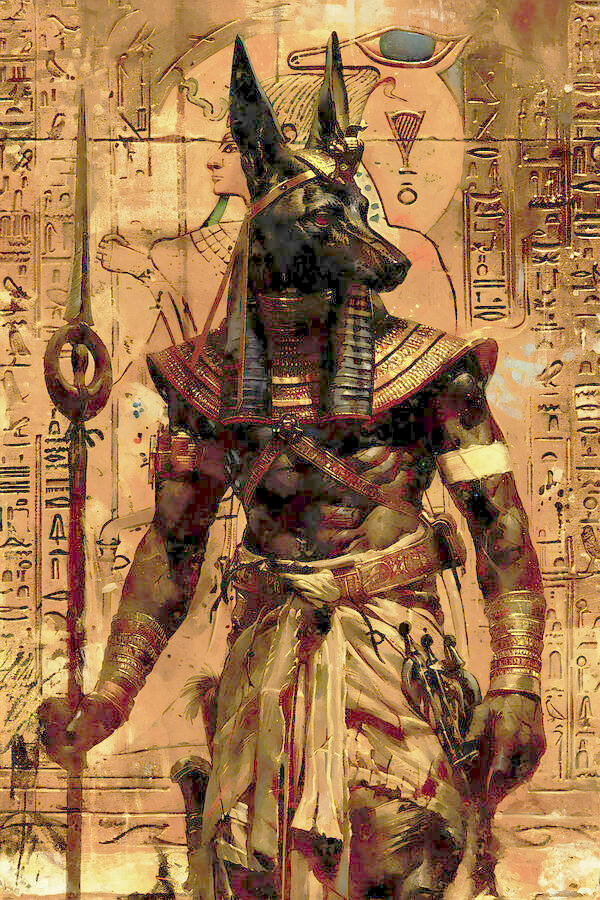
\includegraphics[width=0.2\textwidth]{anub1_edit.png}
};

\node[
    anchor=north west,
    opacity=0.3,      % adjust transparency here
    xshift=-0.3cm,
    yshift=4cm
] at (current page.north west)
{
    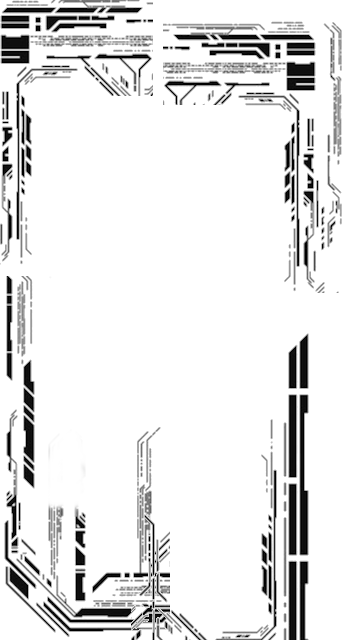
\includegraphics[width=1.6\textwidth]{mepp3.png}
};

\end{tikzpicture}
}

\AddToShipoutPictureFG{
}

% Margins
\geometry{
  top=2.5cm,
  bottom=2.5cm,
  left=3cm,
  right=3cm
}

% Sections style
\titleformat{\section}
{\LARGE\scshape\color{accent}}
{}
{0em}
{}
[\titlerule]

% Commands
\newcommand{\ornament}{
\begin{center}
{\color{gold}
\begin{tikzpicture}
\draw[line width=0.5pt]
(-3,0) -- (3,0);
\filldraw (0,0) circle (2pt);
\end{tikzpicture}}
\end{center}
}

% Center footer

\fancyfoot[C]{
\vspace{-0.3cm}

{\color{gold}
\begin{tikzpicture}
\draw[line width=0.4pt]
(-2.5,0) -- (2.5,0);
\filldraw (0,0) circle (1.5pt);
\end{tikzpicture}
}

\vspace{0.15cm}

{\small\scshape\color{accent}
\thepage}
}

% Left footer
\fancyfoot[L]{
\footnotesize
\color{accent!80}
\texttt{Johnny Teichter}\\
\texttt{0722127856}\\
\texttt{teichohn@gmail.com}
}


\begin{document}
\begin{center}

\begin{tikzpicture}

% =========================
% OUTER FRAME (manuscript border)
% =========================
%\draw[gold, line width=0.6pt]
%(-6,0) rectangle (6,2);

% inner refinement frame
\draw[gold!60, line width=0.6pt]
(-6.21,0.58) rectangle (6.21,2.82);

% =========================
% SIDE ORNAMENT STRIP (very subtle)
% =========================
\fill[gold!20] (-6.2,0.6) rectangle (-5.8,2.8);
\fill[gold!20] (5.4,0.6) rectangle (6.2,2.8);

% engraved dots (left)
\foreach \y in {0.5,0.9,...,2.7} {
    \fill[gold!60] (-6.0,\y) circle (0.6pt);
}

% engraved dots (right)
\foreach \y in {0.5,0.9,...,2.7} {
    \fill[gold!60] (6.0,\y) circle (0.6pt);
}

% =========================
% CENTRAL PLATE (parchment inset)
% =========================
\fill[paper!98]
(-5.8,0.6) rectangle (5.8,2.8);

% subtle inner shadow (depth illusion)
\fill[black!10, opacity=0.08]
(-5.2,0.35) rectangle (5.2,0.35);

% =========================
% TOP DECORATIVE LINE
% =========================
\draw[gold!70, line width=0.8pt]
(-4.5,2.5) -- (4.5,2.5);

% small central ornament
\fill[gold] (0,2.5) circle (1.2pt);

% =========================
% TITLE TEXT
% =========================
\node at (0,1.8)
{\Huge\scshape\color{accent} IT SPECIALIST};

% =========================
% SUBTITLE (refined, not loud)
% =========================
\node at (-0.2,1.05)
{\small\scshape\color{gold!80}
Development \textbullet{} Infrastructure \textbullet{} Security};

% =========================
% BOTTOM LINE (balance)
% =========================
%\draw[gold!60, line width=0.6pt]
%(-4.5,0.45) -- (4.5,0.45);

\end{tikzpicture}
\end{center}
\section*{Chronological Experience}
\textbf{Lead Developer -- Enclave AB 2025--2026}\\
Building a souvereign cloud stack in Kubernetes on Proxmox\\
Complete responsibility of infrastructure design and choices\\[0.4cm]
\textbf{Penetration Tester Student -- ITHS 2024--2026}\\
Vulnwandering in AD environments, penetration testing of web applications,
API consumption with scripting; secure configurations of servers, workstations and OSes\\
Security assessment, Netsec and attack path mapping reporting\\[0.4cm]
\textbf{Customers Service Agent -- Mekonomen Group 2024}\\
Intern due to hireing stop and I just wanted to feel I had a job\\[0.4cm]
\textbf{Technical Repair Shop Assistant -- Alina Service 2024}\\
Trial work week in role selection process. Did memtest, refurbish of hardware,
software reinstallations/updates/fixes + cashier work\\[0.4cm]
\textbf{Search Engine Result Analyst -- OneForma 2023}\\
Analysing data bulks from Google and Bing engines and ranking results
based on relevance and locality of the queries\\[0.4cm]
\textbf{Javascript Algorithms and Data Structures -- freeCodeCamp 2022}\\
Online course corresponding to 300 study hours\\
\newpage

% Page 2 settings

\AddToShipoutPictureBG*{
\begin{tikzpicture}[remember picture,overlay]
\node at (current page.center){

\includegraphics[
width=\paperwidth,
height=\paperheight
]{papier-hintergrund-textur-pergament.jpg}
};
\fill[white,opacity=0.25]
(current page.south west)
rectangle
(current page.north east);
\node[
    anchor=south west,
    opacity=0.3,      % adjust transparency here
    xshift=2.8cm,
    yshift=2cm
] at (current page.south west)
{
    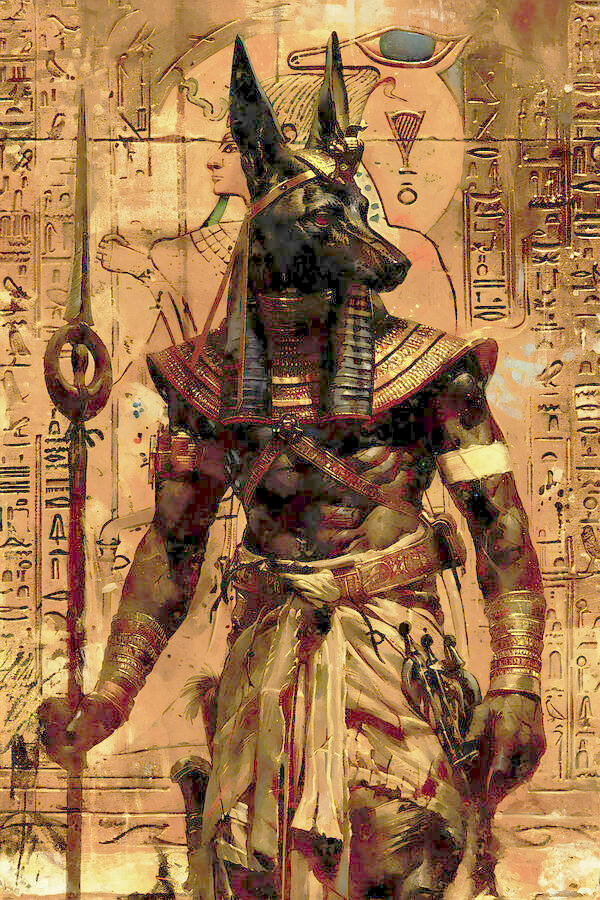
\includegraphics[width=0.2\textwidth]{anub1_edit.png}
};

\node[
    anchor=north west,
    opacity=0.3,      % adjust transparency here
    xshift=-0.3cm,
    yshift=4cm
] at (current page.north west)
{
    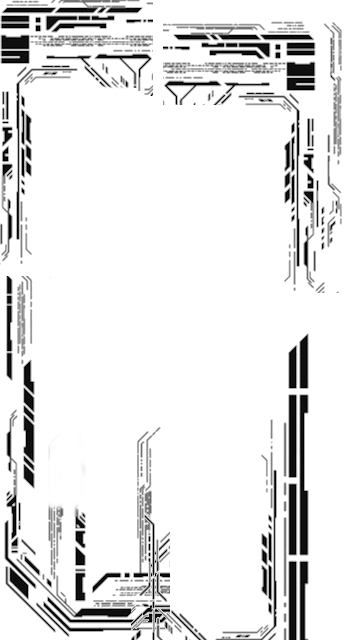
\includegraphics[width=1.6\textwidth]{mepp9.png}
};

\end{tikzpicture}
}

\section*{Relevant Skills}
\textbf{Programming Languages -- C, C++}\\
Written small helper bins in C, a text-based terminal game with keyboard events, and payloads for WinAPI\\[0.4cm]
Developed a Raytracer in C++ with a friend\\ 
Learning game engine development in the OGRE\\[0.4cm]
\textbf{Scripting Languages -- Python, JavaScript, Bash}\\
Built a toolbox of good-use Python scripts to scan network, MiTM ops, handle client--server file transactions,
+ different types of API consumers, scrapers and simple Flasks with login guard\\[0.4cm]
Bash scripting for system maintenance -- Systemd services configs, watchdogs to OOM guard buggy servers, one-click backup locator and restore scripts,
custom changes to application runtimes for separate workspaces and sessions, data sorters and file edits.\\[0.4cm]
\textbf{Frameworks -- AI Agentics, NodeJS + React}\\
Used AI Agentics to configure and setup AI agents for the product of Enclave\\
Implemented a hard-lock system with password protection to guard sensitive files and information, session management and handling of subagent tasks and runtime.\\
Did security research on default settings of the framework and found prompt injection via simple text files.\\
Doing further research on PDF embeddings to test Agentics + RAG systems on this.\\[0.4cm]
Made a typical E-commerce Web portal with a product gallery, checkout cart and admin login for account management in NodeJS + React.
Also played with three.js lib to render animations and made a fun book that opens with camera zoom on content.\\[0.4cm]
\textbf{Markup Languages -- HTML5, CSS, YAML, TeX, XML}\\
Read most of it fluently and TeX is just a new hobbie to learn about different file formats and embeddings of such\\[0.4cm]
\textbf{Human Languages -- Swedish, English}\\[0.4cm]
\end{document}
